\documentclass[12pt]{article}
\usepackage{epsfig}
\usepackage{amssymb}
\usepackage{fullpage}
\usepackage{color}
\usepackage{url}
\usepackage{natbib}
%\usepackage{emulateapj}
\usepackage{footnote}
%\usepackage{deluxetable}

\newcommand{\oii}{[O~{\sc ii}]}
\newcommand{\oiilam}{[O~{\sc ii}]~\ensuremath{\lambda\lambda3726,29}}
\newcommand{\apj}{ApJ}
\newcommand{\pasp}{PASP}
\newcommand{\apjs}{ApJS}
\newcommand{\TODO}[1]{{\it \color{red} (#1)}}

\begin{document}
\title{
  Simulating Emission-Line Galaxy (ELG) Spectra for DESI 
}

\author{John Moustakas (Siena)}
\maketitle

%\abstract{ This technote documents the construction of the preliminary
%  (currently v1.2) emission-line galaxy (ELG) templates for DESI.  }

\section{Introduction}

This document describes the methodology (and code) which was developed
to generate simulated galaxy templates for emission-line galaxies
(ELGs).  The principle purpose of these templates is to facilitate
end-to-end spectral simulations for DESI, although there are many
other potential applications (e.g., optimizing target selection).

This note builds upon the original (static) set of ELG templates
documented in {\tt
  DESI-doc-870-v1}\footnote{https://desi.lbl.gov/DocDB/cgi-bin/private/RetrieveFile?docid=870;filename=elg-templates.pdf;version=1},
which describes the first set of templates.



DESI will obtain high-resolution, observed-frame optical spectroscopy
of four broad classes of objects: quasars (QSOs), emission-line
galaxies (ELGs), luminous red galaxies (LRGs), and stars.  Reliable
spectral templates are critical for several key aspects of the
Project, including spectral simulations (constructing mock datasets),
optimization of targeting strategies, redshift fitting, spectral
classification, and other applications.

The general requirements on the spectral templates for all four
classes of objects are: (1) broad coverage of physical parameter
space; (2) wide wavelength coverage (minimum rest-frame
$\approx0.15-1~\mu$m spectral coverage); (3) high spectral
resolution (at least $\mathcal{R}\approx4500$); and (4) high
spectrophotometric fidelity.  

This document describes the construction of the \emph{preliminary} ELG
templates for DESI.  These templates were constructed from DEEP2/DR4
photometry and spectroscopy of a large sample of galaxies at $z\sim1$
with measurable \oiilam{} nebular emission and extensive broadband
photometric coverage.

\section{DEEP2 Observations}

The DEEP2 Galaxy Redshift Survey (hereafter, DEEP2) obtained
high-resolution optical spectroscopy of more than $50,000$
intermediate-redshift galaxies using the DEIMOS multi-object
spectrograph on the Keck~2 telescope \citep{newman13a}.  DEEP2
spectroscopy spans the $\approx6500-9300$~\AA{} observed-frame
wavelength range at a resolution of $R\approx6000$ with $0.33$~\AA{}
pixels.  With this instrumental setup, DEEP2 spectroscopy resolved the
\oiilam{} nebular emission-line doublet for galaxies at
$z\approx0.7-1.4$.

The public DEEP2 data were retrieved and pre-processed in the
following way:\footnote{Note that not all of the {\sc idl} code
  alluded to in this document is checked into the DESI {\sc svn}
  repository because it is part of my personal research code.
  However, all of this code can be inspected or retrieved from my
  public {\tt GitHub} repository:
  \url{https://github.com/moustakas/moustakas-projects} (see
  especially the {\tt deep2} and {\tt desi} directories).}

%Redshift and photometric catalogs, as well as 1D and 2D spectra were
%retrieved from the DEEP2 fourth public data release (DR4)
%website\footnote{\url{http://deep.ps.uci.edu/dr4}} as described
%below:

\begin{enumerate}
\item{First, all the redshift and photometric catalogs are downloaded,
  as well as the 1D and 2D spectra which were released as part of the
  fourth public data release (DR4) from
  \url{http://deep.ps.uci.edu/dr4}.  The full DEEP2 redshift catalog
  (including duplicate objects) is called {\tt zcat.deep2.dr4.fits.gz}
  (N=52,989), while the catalog of unique galaxies is called {\tt
    zcat.deep2.dr4.uniq.fits.gz} (N=50,319).  Among the subset of
  unique galaxies, N=35,781 have high-quality spectroscopic redshifts,
  $Q\ge3$ (see \citealt{newman13a} for details).}
\item{The script {\tt deep2\_check\_spec1d\_dr4} runs through the full
  catalog of unique objects, checks the fidelity of the 1D spectra,
  and determines which spectra can be flux-calibrated.\footnote{The
    code and response functions needed to flux-calibrate the DEEP2
    spectra to within $\sim10\%$ is not public but can be requested
    from Jeff Newman (JANewman@pitt.edu).}  This script produces the
  file {\tt zcat.dr4.goodspec1d.Q34.fits.gz} (N=35,682), which
  contains the set of (unique!) objects with $Q\ge3$ whose spectra
  could be flux-calibrated.  Note that this catalog contains $99.8\%$
  of the original sample of unique galaxies.}
\item{Finally, the script {\tt build\_deep2\_photo\_catalog} generates
  a line-matched photometric catalog for this sample by matching
  against the \citet{matthews13a} extended photometric
  catalog.\footnote{On the DEEP2/DR4 website the Matthews extended
    photometric catalog is called {\tt zcat\_ext.uniq.fits.gz}, and
    the matching is done using the {\sc objno} structure tag.}  This
  catalog contains $BRI$ photometry and recalibrated $ugriz$
  photometry from the CFHTLS Wide and Deep surveys.  The overwhelming
  majority of matching objects ($\approx75\%$) have 8-band photometry
  ($ugrizBRI$), while the remainder have just three bands of $BRI$
  photometry.  This script also adds
  unWISE\footnote{\url{http://unwise.me}} W1 and W2 ($3.4$ and
  $4.6~\mu$m) photometry to the sample, based on running {\tt The
    Tractor}\footnote{\url{http://thetractor.org}} in
  forced-photometry mode at the position of all the DEEP2 sources
  brighter than $R=24.1$, as well as morphological information (for
  approximately $10\%$ of the sample) from the Advanced Camera for
  Surveys General Catalog \citep[ACS-GC;][]{griffith12a}.  The output
  file produced by this script is called {\tt
    photo.dr4.goodspec1d.Q34.fits.gz} (N=35,682).}
\end{enumerate}

%The 'zcat.dr4.goodspec1d.Q34.fits.gz' redshift catalog is used in all
%my subsequent analysis.

\section{DEEP2 Galaxy Modeling}

%\subsection{Emission-line fitting}

With the redshift and photometric catalogs described above in hand, as
well as the corresponding 1D spectra, the following procedure is
carried out to model the data:

\begin{itemize}
\item{First, the 1D spectra of all 35,682 objects in the {\tt
    zcat.dr4.goodspec1d.Q34.fits.gz} catalog are fitted using the
  stellar continuum and emission-line fitting code described in
  \citet{moustakas10a}.  The spectra are fitted twice, first by
  allowing the \oiilam{} doublet ratio to be free, and a second time
  by fixing the \oii~$\lambda3726/$\oii{}~$\lambda3729$ doublet ratio
  to $0.73$ (the median ratio of galaxies in the sample with
  well-measured \oii).  Fixing the doublet ratio ensures that
  lower-S/N \oii{} lines are fitted with two distinct lines, rather
  than one single broad line.  The spectra are fitted using the script
  {\tt deep2\_gandalf\_specfit\_dr4}, which runs on each individual
  DEEP2 mask, and the results are parsed and merged by running the
  scripts {\tt parse\_deep2\_gandalf\_specfit\_dr4} and {\tt
    deep2\_merge\_gandalf\_specfit\_dr4}, in that order.  An emission
  line is considered ``measured'' if the amplitude of the line is
  $>1.5$ times above the {\sc rms} of the surrounding continuum.  If
  an emission line is not detected based on this criterion then a
  $1\sigma$ upper limit is computed.  The output emission-line catalog
  is called {\tt deep2.ppxf.specdata.dr4\_v1.0.fits.gz} (N=35,682).
  Finally, the same scripts are run with the {\tt /fixoii} keyword,
  which generates the corresponding {\tt
    deep2.ppxf.specdata.fixoii.dr4\_v1.0.fits.gz} (N=35,682) catalog.}
     
\item{Next, the $ugrizBRI$ plus unWISE $3.4$ and $4.6~\mu$m broadband
  photometry of the sample are fitted using the Bayesian spectral
  energy distribution (SED) modeling code {\tt iSEDfit}
  \citep{moustakas13a}.\footnote{\url{https://github.com/moustakas/impro}}
  The script used to do the actual fitting is called {\tt
    desi\_deep2\_isedfit}.  A fiducial set of prior parameters are
  adopted, as well as the
  FSPS\footnote{\url{https://www.cfa.harvard.edu/~cconroy/FSPS.html}}
  \citep[v2.4;][]{conroy09a, conroy10b} spectral synthesis models
  based on the MILES\footnote{\url{http://miles.iac.es}} stellar
  library, which has a resolution of approximately $2.5$~\AA{} FWHM
  ($\mathcal{R}\approx2200$) between $3600-7500$~\AA; outside this
  spectral range the FSPS models are based on the BaSeL stellar
  library, which has a FWHM resolution of roughly $20$~\AA{} FWHM.
  The output {\tt iSEDfit} catalog is called {\tt
    desi\_deep2\_fsps\_v2.4\_miles\_chab\_charlot\_sfhgrid01.fits.gz}
  (N=35,682).  In addition, the best-fitting (maximum likelihood) SEDs
  are used to compute $K$-corrections, and to estimate the mean
  continuum flux around $3727$~\AA{} (rest), producing the catalog
  {\tt
    desi\_deep2\_fsps\_v2.4\_miles\_chab\_charlot\_sfhgrid01\_kcorr.z0.0.fits.gz}
  (N=35,682).}

\item{The final step in this process combines the spectroscopic
  (emission-line) and photometric (SED) galaxy modeling results.  The
  {\tt desi\_deep\_isedfit} script with the {\tt /build\_oiiflux}
  keyword set generates a master, line-matched catalog of integrated
  \oii{} fluxes for the sample using the technique described in
  \citet{zhu09a}.  Briefly, the \oii{} emission-line equivalent width
  (EW) measured for each galaxy is scaled by the continuum flux around
  $3727$~\AA{} (rest) inferred from the SED modeling, resulting in
  integrated \oii{} fluxes in erg~s$^{-1}$~cm$^{-2}$ for all the
  galaxies were \oii{} could be measured (or where an upper limit
  could be computed).  The output catalog produced by this script is
  called {\tt deep2\_oiicat\_VERSION.fits.gz} (N=35,682), where {\tt
    VERSION} is the template version number.}
\end{itemize}

%In addition, although the DEEP2 spectra have been flux-calibrated to
%within $\sim10\%$, we still need to account for slit-losses.  I used
%the technique described in \citet{zhu09a} to estimate the [OII]
%emission-line flux in physical units.

\section{ELG Templates}

%Note that the instrumental resolution of the DEEP2/DEIMOS spectra is
%R~6000 between ~6500-9100 A.

%\begin{deluxetable}{ll}
%\tablecaption{Rest-frame ELG Template Parameters\label{table:rest}} 
%\tablewidth{0pt}
%\tablehead{
%\colhead{Parameter} & \colhead{Value}
%}
%\startdata
%Number of templates     & $7876$ \\
%Number of pixels        & $31,171$ \\ 
%Rest-frame wavelength range & $0.125-1.0~\mu$m (vacuum) \\
%Spectral resolution (emission lines) & Effectively infinite \\
%Spectral resolution (continuum) & $\approx2200$ \\
%Pixel size & $20$~km~s$^{-1}$ \\
%Flux units & erg~s$^{-1}$~cm$^{-2}$~\AA$^{-1}$ at $10$~pc
%\enddata
%%\tablenotetext{a}{Cluster coordinates based on the position of the BCG.}
%\end{deluxetable}

The ELG templates are constructed by combining the SEDs inferred from
modeling the broadband photometry with the \oii{} emission-line
profile and line-strength inferred from the DEEP2 spectroscopy.  The
script {\tt build\_desi\_elg\_templates} generates the actual ELG
templates from the parent sample of 35,682 DEEP2 galaxies.  First, a
subset of galaxies suitable for template-building are identified by
applying the following cuts:

\begin{enumerate}
\item[$\bullet$]{$0.75<z<1.45$;}
\item[$\bullet$]{$r_{\rm CFHTLS}<23.5$ (AB, extinction-corrected);}
\item[$\bullet$]{minimum 6 bands of observed-frame optical photometry;}
\item[$\bullet$]{\oiilam{} doublet measured with ${\rm S/N}>3$; and}
\item[$\bullet$]{EW(\oii)$>1$~\AA.}
\end{enumerate}

These cuts leave a total of $7876$ galaxies, the most stringent cut
being on the S/N of the \oii{} doublet.  Next, the \oii{} line-profile
and integrated flux for each galaxy is used as an anchor to construct
a more complete nebular emission-line spectrum.  Briefly, the nebular
emission-line model implemented within {\tt iSEDfit} is used to add
more than $50$ additional emission lines.  The strengths of the
hydrogen and helium recombination lines are based on the number of
hydrogen-ionizing photons inferred from the SED modeling, while the
forbidden emission-line strengths are based on empirically determined
line-ratios.

With these empirically constrained broadband SEDs and nebular
emission-line spectra in hand, a set of rest-frame and observed-frame
templates are generated.  Tables~\ref{table:rest} and \ref{table:obs}
summarize the spectral parameters of the rest-frame and observed-frame
templates, respectively.  The principle difference between the two
template sets is that the rest-frame templates have
constant-$\log_{10}(\lambda)$ ($20$~km~s$^{-1}$) pixels, while the
observed-frame templates have constant-$\lambda$ ($0.5$~\AA) pixels.
In addition, the rest-frame templates are normalized to a
$1~M_{\odot}$ (stellar masss) stellar population at $10$~pc, while the
observed-frame templates retain the redshift and flux normalization of
the corresponding DEEP2 galaxy.

%Include some figures:
%* color-redshift plots
%* many other ideas

%\begin{deluxetable}{ll}
%\tablecaption{Observed-frame ELG Template Parameters\label{table:obs}} 
%\tablewidth{0pt}
%\tablehead{
%\colhead{Parameter} & \colhead{Value}
%}
%\startdata
%Number of templates     & $7876$ \\
%Number of pixels        & $15,001$ \\ 
%Rest-frame wavelength range & $0.35-1.1~\mu$m (vacuum) \\
%Spectral resolution (emission lines) & Effectively infinite \\
%Spectral resolution (continuum) & $\approx2200$ \\
%Pixel size & $0.5$~\AA \\
%Flux units & erg~s$^{-1}$~cm$^{-2}$~\AA$^{-1}$\\
%\enddata
%%\tablenotetext{a}{Cluster coordinates based on the position of the BCG.}
%\end{deluxetable}

\section{Ancillary Information}

The code used to generate this preliminary set of observed- and
rest-frame ELG templates has been checked into the DESI {\sc svn}
repository in {\tt code/spectro/templates/elg\_templates}.  The
templates can be found on NERSC in {\tt
  \$\{DESI\_ROOT\}/spectro/templates/elg\_templates/VERSION}, where
{\tt VERSION} is the template version number (currently v1.2).  

The rest-frame template file, {\tt elg\_templates\_VERSION.fits.gz},
is a binary FITS table with two extensions:

\begin{enumerate}
\item{Extension~0: An [{\sc npixel}]$\times$[{\sc ntemplate}] flux
  array which contains {\sc ntemplate} spectra, each {\sc npixel}
  pixels long (see Table~\ref{table:rest} above).}
\item{Extension~1: An [{\sc ntemplate}] data structure with the
  following metadata:
\begin{itemize}
\item{.{\sc TEMPLATEID} - unique template ID number (zero-indexed)}
\end{itemize}
}
\end{enumerate}

The observed-frame template file, {\tt
  elg\_templates\_obs\_VERSION.fits.gz}, is a binary FITS table with
two extensions:

\begin{enumerate}
\item{Extension~0: An [{\sc npixel}]$\times$[{\sc ntemplate}] flux
  array which contains {\sc ntemplate} spectra, each {\sc npixel}
  pixels long (see Table~\ref{table:obs} above).}
\item{Extension~1: An [{\sc ntemplate}] data structure with the
  following metadata:
\begin{itemize}
\item{.{\sc TEMPLATEID} - unique template ID number (zero-indexed)}
\item{.{\sc OBJNO} - unique DEEP2 identifier}
\item{.{\sc RA} - right ascension (degrees, J2000)}
\item{.{\sc DEC} - declination (degrees, J2000)}
\item{.{\sc Z} - heliocentric redshift of the DEEP2 galaxy} 
\item{.{\sc SIGMA\_KMS} - intrinsic velocity line-width (km/s)} 
\item{.{\sc OII\_3726} - \oii~$\lambda3726$ emission-line flux
  (erg~s$^{-1}$~cm$^{^2}$)}  
\item{.{\sc OII\_3729} - \oii~$\lambda3729$ emission-line flux
  (erg~s$^{-1}$~cm$^{^2}$)} 
\item{.{\sc OII\_3727} - total \oiilam{} emission-line flux
  (erg~s$^{-1}$~cm$^{^2}$)} 
\item{.{\sc OII\_3727\_EW} - rest-frame \oii~$\lambda3726,29$
  equivalent width (\AA)}
\item{.{\sc RADIUS\_HALFLIGHT} - half-light radius (arcsec) ($-999$ if not measured)}
\item{.{\sc SERSICN} - Sersic n parameter (concentration) ($-999$ if not measured)}
\item{.{\sc AXIS\_RATIO} - minor-to-major axis ratio ($-999$ if not measured)}
\item{.{\sc DECAM\_G} - synthesized DECam g-band AB magnitude}
\item{.{\sc DECAM\_R} - synthesized DECam r-band AB magnitude}
\item{.{\sc DECAM\_Z} - synthesized DECam z-band AB magnitude}
\item{.{\sc LOGMSTAR} - log10(stellar mass) ($M_{\odot}$, $h=0.7$,
  \citealt{chabrier03a} IMF)} 
\item{.{\sc LOGSFR} - log10(star formation rate)
  ($M_{\odot}$~yr$^{-1}$, $h=0.7$, \citealt{chabrier03a} IMF)}
\item{.{\sc AV\_ISM} - $V$-band continuum attenuation (mag,
  \citealt{charlot00a} attenuation curve)} 
\end{itemize}
}
\end{enumerate}

\section{Future Improvements}

Future improvements to these templates may include (in no particular
order): 

\begin{enumerate}
\item{Extending the spectral coverage redward into the mid-infrared so
  that WISE photometry can be synthesized from the models.}
\item{Including additional nebular emission lines.}
\item{Constructing a smaller basis set of models (e.g., archetypes)
  which adequately span the physical parameter space of the full set
  of templates.}
\item{Incorporate more intelligent resampling of the data and models,
  in order to ensure that flux is being conserved correctly.}
\item{Expanding this TechNote to include more quantitative tests of
  the models (e.g., how well they span color-color and color-redshift
  space relative to actual observations).}
\end{enumerate}

\section{Note regarding previous versions}

This TechNote describes the construction of the v1.2 ELG templates.
The most significant updates with respect to previous undocumented
versions (v1.0 and v1.1) is the construction of both observed-frame
and rest-frame templates, the addition of size and morphology
measurements based on HST imaging for approximately $10\%$ of the
sample, and a number of (significant!) bug fixes.  Also note that the
previous versions of ELG templates are not backwards-compatible with
the current version!

\begin{figure}
\centering
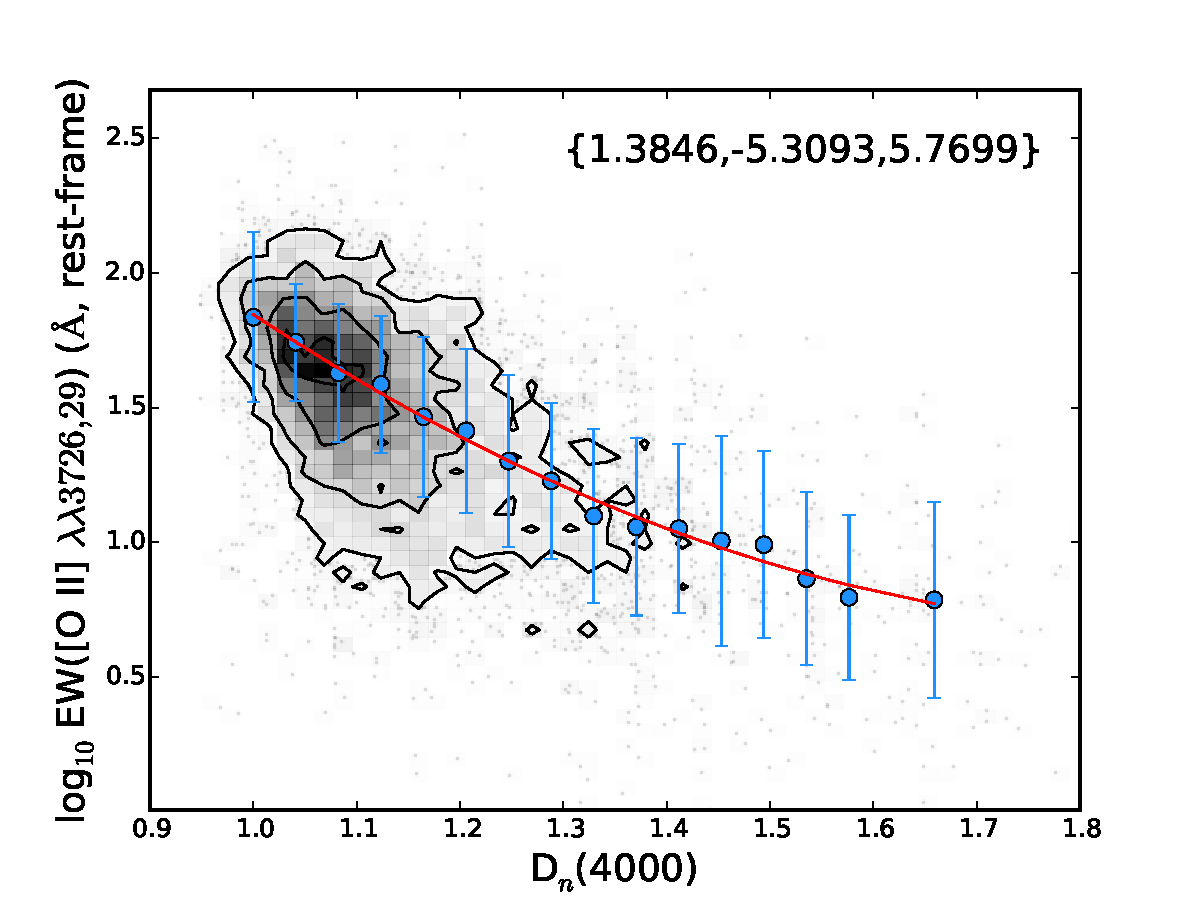
\includegraphics[width=0.8\textwidth]{figures/d4000_ewoii.pdf}
\caption{Rest-frame \oii{} equivalent width vs.~the $4000$-\AA{}
  break, $D_{n}(4000)$.  The blue points and uncertainties indicate
  the running median and standard deviation in $0.05$-wide bins of
  $D_{n}(4000)$, while the red curve is a third-order polynomial fit
  to the points with the coefficients given in the
  legend.  The dispersion is relatively uniform with $D_{n}(4000)$
  with a mean value of $0.31$~dex.  \label{fig:d4000}} 
\end{figure}

\bibliographystyle{apj}
\bibliography{/Users/ioannis/bibdesk/ioannis}
%\input{elg-templates.bbl}

\end{document}


